%% 
%% Copyright 2007-2020 Elsevier Ltd
%% 
%% This file is part of the 'Elsarticle Bundle'.
%% ---------------------------------------------
%% 
%% It may be distributed under the conditions of the LaTeX Project Public
%% License, either version 1.2 of this license or (at your option) any
%% later version.  The latest version of this license is in
%%    http://www.latex-project.org/lppl.txt
%% and version 1.2 or later is part of all distributions of LaTeX
%% version 1999/12/01 or later.
%% 
%% The list of all files belonging to the 'Elsarticle Bundle' is
%% given in the file `manifest.txt'.
%% 

%% Template article for Elsevier's document class `elsarticle'
%% with numbered style bibliographic references
%% SP 2008/03/01
%%
%% 
%%
%% $Id: elsarticle-template-num.tex 190 2020-11-23 11:12:32Z rishi $
%%
%%
% \documentclass[preprint,12pt]{elsarticle}

%% Use the option review to obtain double line spacing
% \documentclass[authoryear,preprint,review,12pt]{elsarticle}

%% Use the options 1p,twocolumn; 3p; 3p,twocolumn; 5p; or 5p,twocolumn
%% for a journal layout:
% \documentclass[final,1p,times]{elsarticle}
%% \documentclass[final,1p,times,twocolumn]{elsarticle}
% \documentclass[final,3p,times]{elsarticle}
\documentclass[final,3p,times,onecolumn]{elsarticle}
%% \documentclass[final,5p,times]{elsarticle}
% \documentclass[final,5p,times,twocolumn]{elsarticle}

%% For including figures, graphicx.sty has been loaded in
%% elsarticle.cls. If you prefer to use the old commands
%% please give \usepackage{epsfig}

%% The amssymb package provides various useful mathematical symbols
\usepackage{amssymb}
\usepackage[UTF8]{ctex}
\usepackage{graphicx}
%% The amsthm package provides extended theorem environments
%% \usepackage{amsthm}

%% The lineno packages adds line numbers. Start line numbering with
%% \begin{linenumbers}, end it with \end{linenumbers}. Or switch it on
%% for the whole article with \linenumbers.
%% \usepackage{lineno}

\journal{Mathematical thesis}

\begin{document}

\begin{frontmatter}

%% Title, authors and addresses

%% use the tnoteref command within \title for footnotes;
%% use the tnotetext command for theassociated footnote;
%% use the fnref command within \author or \address for footnotes;
%% use the fntext command for theassociated footnote;
%% use the corref command within \author for corresponding author footnotes;
%% use the cortext command for theassociated footnote;
%% use the ead command for the email address,
%% and the form \ead[url] for the home page:
%% \title{Title\tnoteref{label1}}
%% \tnotetext[label1]{}
%% \author{Name\corref{cor1}\fnref{label2}}
%% \ead{email address}
%% \ead[url]{home page}
%% \fntext[label2]{}
%% \cortext[cor1]{}
%% \affiliation{organization={},
%%             addressline={},
%%             city={},
%%             postcode={},
%%             state={},
%%             country={}}
%% \fntext[label3]{}

\title{关于隔项有零数列通项公式的研究}

%% use optional labels to link authors explicitly to addresses:
%% \author[label1,label2]{}
%% \affiliation[label1]{organization={},
%%             addressline={},
%%             city={},
%%             postcode={},
%%             state={},
%%             country={}}
%%
%% \affiliation[label2]{organization={},
%%             addressline={},
%%             city={},
%%             postcode={},
%%             state={},
%%             country={}}

\author{赵文瑞}

\author{王心雨}

\address{organization={天津市耀华中学},%Department and Organization
            addressline={天津市和平区南京路106号}, 
            city={天津},
            postcode={300000}, 
            state={学生},
            country={中国}}

\begin{abstract}

%% Text of abstract
探究一种隔项有n个0数列的通项公式并探索构造此类函数的函数,推广至所有常规周期数列。

\end{abstract}

%%Graphical abstract
% \begin{graphicalabstract}
%\includegraphics{grabs}
% \end{graphicalabstract}

%%Research highlights
% \begin{highlights}
% \item Research highlight 1
% \item Research highlight 2
% \end{highlights}

\begin{keyword}

$\qquad$数列,\:通项公式,\:隔项有零数列,\:周期性,\:傅里叶级数,\:复数,\:频率,\:原神,\:三角函数,\:欧拉公式
%% keywords here, in the form: keyword \sep keyword

%% PACS codes here, in the form: \PACS code \sep code

%% MSC codes here, in the form: \MSC code \sep code
%% or \MSC[2008] code \sep code (2000 is the default)

\end{keyword}

\end{frontmatter}

%% \linenumbers

\section*{引言}

数列是我们研究离散数学的一个非常重要的工具,作为周期数列基础的隔项有零数列,其递推公式非常容易,但对其通项公式我们却不太容易描述。

如果可以找到一种函数,确定此种数列的所有参数,输出其数列的通项公式,就可以快速找到任意隔项有零数列(周期数列)的通项公式。

无疑这种函数也应当是周期性的函数,说到周期性函数我们首先想到的一定三角函数,但在其最小正周期中的函数值变化规律还是三角函数,也就是说我们较难找到使三角函数准确贴合我们需要数列通项公式条件的改变方法,那么我们不妨使用另一种工具来实现类似三件函数的周期性。

感谢徐健坤同学在2节和4.1节对本文的帮助。

\newpage

\tableofcontents

\newpage

%% main text
\section{数列}

\subsection{数列定义}

\textbf{数列}是由数字组成的序列,也就是以正整数系为定义域,值域包含于某数系的函数。

\subsection{通项公式}

如果数列${a_n}$的第n项$a_n$与n之间的关系可以用一个公式来表示,这个公式叫做数列的通项公式(general formulas)。

\subsection{特殊数列}

\subsubsection{等差数列}

数列中，从第二项起，每一项与前一项的差相等。

例如数列${\displaystyle 1,3,5,7,9,\cdots ,9995,9997,9999,\cdots }1,3,5,7,9,\cdots ,9995,9997,9999,\cdots$。

若设首项$a_{1}=a$,则等差数列的通项公式为$a_{n}=a_{1}+(n-1)d$。

\subsubsection{等比数列}

它的特点是：从第2项起,每一项与前一项的比都是一个常数。

例如数列$2,4,8,16,32,\cdots ,2^{197},2^{198},2^{199},\cdots$。

若设首项$a_{1}=a$,则等比数列的通项公式为$a_{n}=ar^{n-1}$。

\subsubsection{斐波那契数列}

它的特点是：从第2项起,每一项与前一项的比都是一个常数。

以数学符号表示，即$a_{1}=a_{2}=1$,且对于$n\geq 3$,$a_{n}=a_{n-1}+a_{n-2}$。

斐波那契数列的通项公式为$a_{n}={\frac {1}{\sqrt {5}}}[({\frac {1+{\sqrt {5}}}{2}})^{n}-({\frac {1-{\sqrt {5}}}{2}})^{n}]$。

\section{隔项有零数列}

常指在常数列所有相邻两项之间插入一个0(首项前可选插入一个0)形成的数列。

\subsection{隔项有零数列的形式}

形如: $n,0,n,0,n,0,n,0,\cdots$。

或: $0,n,0,n,0,n,0,n,\cdots$的数列我们可以称其为隔项有零数列。

\subsection{隔项有零数列的递推公式}

设原常数列通项公式为c。

$\{a_n\}$前两项为0,c或c,0。

$$a_n=a_{n-2}\qquad(n>2)$$

这也说明了隔项有零数列是周期数列。

\subsection{隔项有零数列的通项公式}

设原常数列通项公式为c。

$$a_n=\frac{c}{2}[(-1)^n+1]\qquad(n\rightarrow(n-1))$$

或

$$a_n=c|\sin\frac{n\pi}{2}|\qquad(n\rightarrow(n-1))$$

\section{隔项有n零的数列}

明白了上面的隔项有一个零的数列和其通项公式,我们不禁联想到如果一个常数列所有相邻项中插入一个0形成的数列(首项前插入0的个数小于相邻项之间的),也就是隔项有n个零数列(n>0),那么这种数列的通项公式是什么呢?

\subsection{设想形式}

可以想到,这是一个形如:$\underbrace{0,0,\cdots,0,0}_{(n-p)*0},1,\underbrace{0,0,\cdots,0,0}_{n*0},1,\underbrace{0,0,\cdots,0,0}_{n*0},1,\cdots$(p$<$n)的数列。

\subsection{对比}

对于隔项有一个零的数列的通项公式,我们很容易找到一个q(n),使其输出值随n以1为增量的递增而在0和c之间来回变换。

那对于隔项有n个0的通项公式,其函数也应满足一定条件,使其输出值随n以1为增量的递增而输出我们需要的周期性数列。

\subsection{目标函数}

如果这个数列每k(收敛)项可以形成一个最小周期,原常数列通项公式c,相位为p。

我们可以设想一下这个关于n-p的函数满足什么条件,可以想到在输入值为正整数时函数的值域属于\{0,1\},并且在函数等于c之后,n再递增k次后函数的值又为c,在输入值为正整数且输出值不为c时输出值为0。

\subsection{可能的函数或方法}

以下列举了一些我们认为最有可能的函数或方法:

\subsubsection{三角函数}

三角函数的周期性非常符合周期数列通项公式的性质,不过因为三角函数周期内(非最小周期)极点均匀交错排布,使最小值之间的距离与最小值和最大值之间的距离不等,需要进行周期性不均匀缩放或是改用非最小值点作为零点,较难变成目标函数,所以并未采取这种方法。

\subsubsection{傅里叶逆变换}

作为一个周期性函数,根据三角函数的正交性,其傅里叶级数展开为$\frac{a_0}{2}+\sum\limits_{n=1}^\infty (a_ncosnx+b_nsinnx)$的形式。

如果可以找到三角函数的叠加对新周期函数极值影响的规律,那么运用傅里叶逆变换则可以得到所求函数,但是因为傅里叶变换普遍运用于去除或添加某频率的周期函数,对新函数的各种性质的预测并不准确,且周期函数的加和与目标函数的差距难以量化,所以并未采取这种方法。

\subsubsection{复数}

通过3.2我们了解了隔项有一个零数列通项公式,不妨深入理解一下。

$(-1)^n$的值随着n以增值为1的递增而从-1和1之间来回切换,我们不妨引入复平面,复平面的0点在一个模长为1的向量的起点,向量的终点落在-1处。

这个向量随着n以增值为1的递增不断以0点为中心旋转,每次递增顺时针旋转,每旋转两次为一个周期$\pi rad$。

设想可以找到向量$\overrightarrow{\alpha}$,使其进行g(n,$\alpha$)的运算,输出值为此向量绕0点旋转$\frac{2\pi}{k}$个弧度,再通过其他手段使其输出值非1的值变为零(可以在复平面内抵消),之后进行一些简单的线性变换,就可以得到目标函数。

在本文中最终也采取了这种方法。

\section{推导}

以下为推导过程:

\subsection{欧拉公式}

由欧拉公式可知:

$$e^{ix}=\cos x+i\sin x$$

也就是复平面单位圆上的点可以用$e^{ix}$来表示,x为逆时针弧度值,其符合一般数学规律而在运算中相比于n+mi的形式更易理解。

\subsection{复平面单位圆内接正多边形顶点性质}

在复平面单位圆内构造一个正k边形,其中一个顶点落在1处,称为$\zeta_0$,从$\zeta_0$开始以单位圆为路线逆时针路过的顶点依次为$\zeta_1,\zeta_2,\cdots,\zeta_{k-1}$。

根据欧拉公式,我们可易得以下性质:

$m,n\in N$

1. $\zeta_n^m=\zeta_{n\times m}$

$\qquad\because\zeta_n$可表示为$e^{\frac{2\pi in}{k}}$

$\qquad\therefore\zeta_n^m=e^{\frac{2\pi in}{k}^m}=e^{\frac{2\pi inm}{k}}=\zeta_{n\times m}$

2. $\zeta_n=\zeta_{n-k}$

$\qquad e^{\frac{2\pi in}{k}}=e^{\frac{2\pi in}{k}-2\pi i}=e^{\frac{2\pi i(n-k)}{k}}=\zeta_{n-k}$

3. $\zeta_0+\zeta_1+\cdots+\zeta_{k-1}=0$

$\qquad\because$正多边形顶点都在单位元上,可知多k形中心为0点且到所有顶点的距离都为1,设0点到所有顶点的向量和为$\overrightarrow{a}$
将此正k边形绕0点逆时针旋转$\frac{2\pi}{k}$弧度,明显的,$\overrightarrow{a}$也逆时针旋转$\frac{2\pi}{k}$弧度,但向量之和不变。

$\qquad\therefore\overrightarrow{a}=\overrightarrow{0}$

$\qquad\therefore\zeta_0+\cdots+\zeta_{k-1}=0$

4. $\zeta_m^n=1\quad(\frac{n}{k}\in N)$

$\qquad\because\zeta_m^n=e^{\frac{2mn\pi i}{k}}\quad\frac{mn}{k}\in N$

$\qquad\therefore\zeta_m^n={e^{2\pi i}}^{\frac{mn}{k}}=1^{\frac{mn}{k}}=1$

5. $\zeta_0^n+\zeta_1^n+\cdots+\zeta_{k-1}^n=0\quad(\frac{n}{k}\notin N)$

$\qquad\because\zeta=e^{\frac{2\pi}{k}i}\qquad\zeta_j=e^{\frac{2j\pi}{k}i}$

$\qquad\therefore\zeta_j^n=e^{\frac{2jn\pi}{k}}$

$\qquad\therefore\zeta_1=\zeta,\:\zeta_j=\zeta^j$

$\qquad\therefore$

$$\sum\limits_{j=0}^{k-1}\zeta_j^n=\sum\limits_{j=0}^{k-1}\zeta^{jn}=\frac{1-(\zeta^n)^k}{1-\zeta^n}=0$$

\subsection{构造函数}

设目标函数为f(n)

设g(k,p,c)=h,可得:

$$g(k,p,c)=h$$

$$h(x)=\frac{c}{k}\sum\limits_{m=0}^{k-1}e^{\frac{2m\pi\imath (x-p)}{k}}$$

这里我们发现h(x)是一个周期为k的函数,尝试代入数据进行傅里叶级数展开。

以下是周期为5,相位为0,原函数通项公式为1的数列的通项公式:

$$f(n)=1+e^{\frac{2i\pi n}{5}}+e^{\frac{4i\pi n}{5}}+e^{\frac{6i\pi n}{5}}+e^{\frac{8i\pi n}{5}}$$

\newpage

函数图像为(取模长):

\begin{figure}[h]
    \centering
    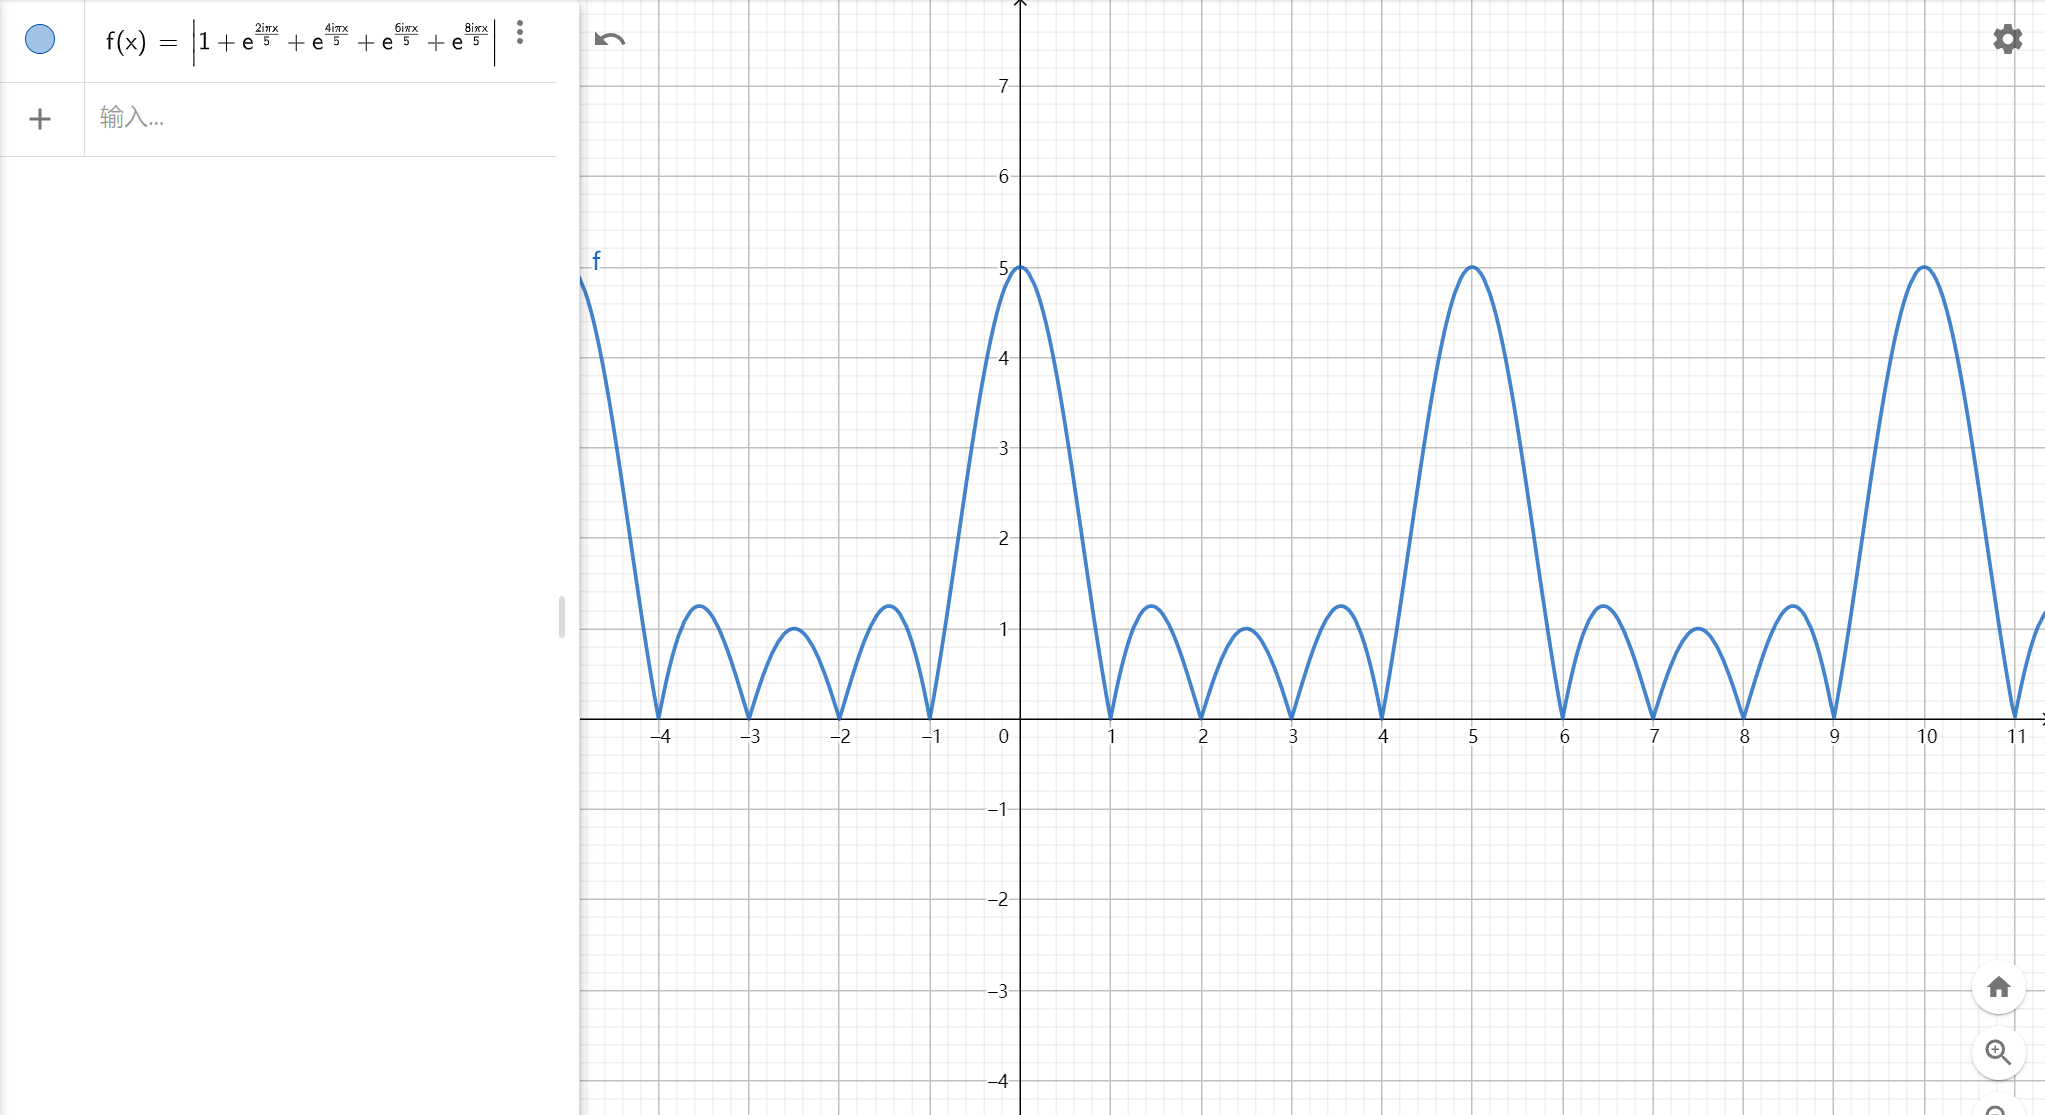
\includegraphics[width=360pt]{func.png}
\end{figure}

其傅里叶级数5阶展开为:

\begin{figure}[h]
    \centering
    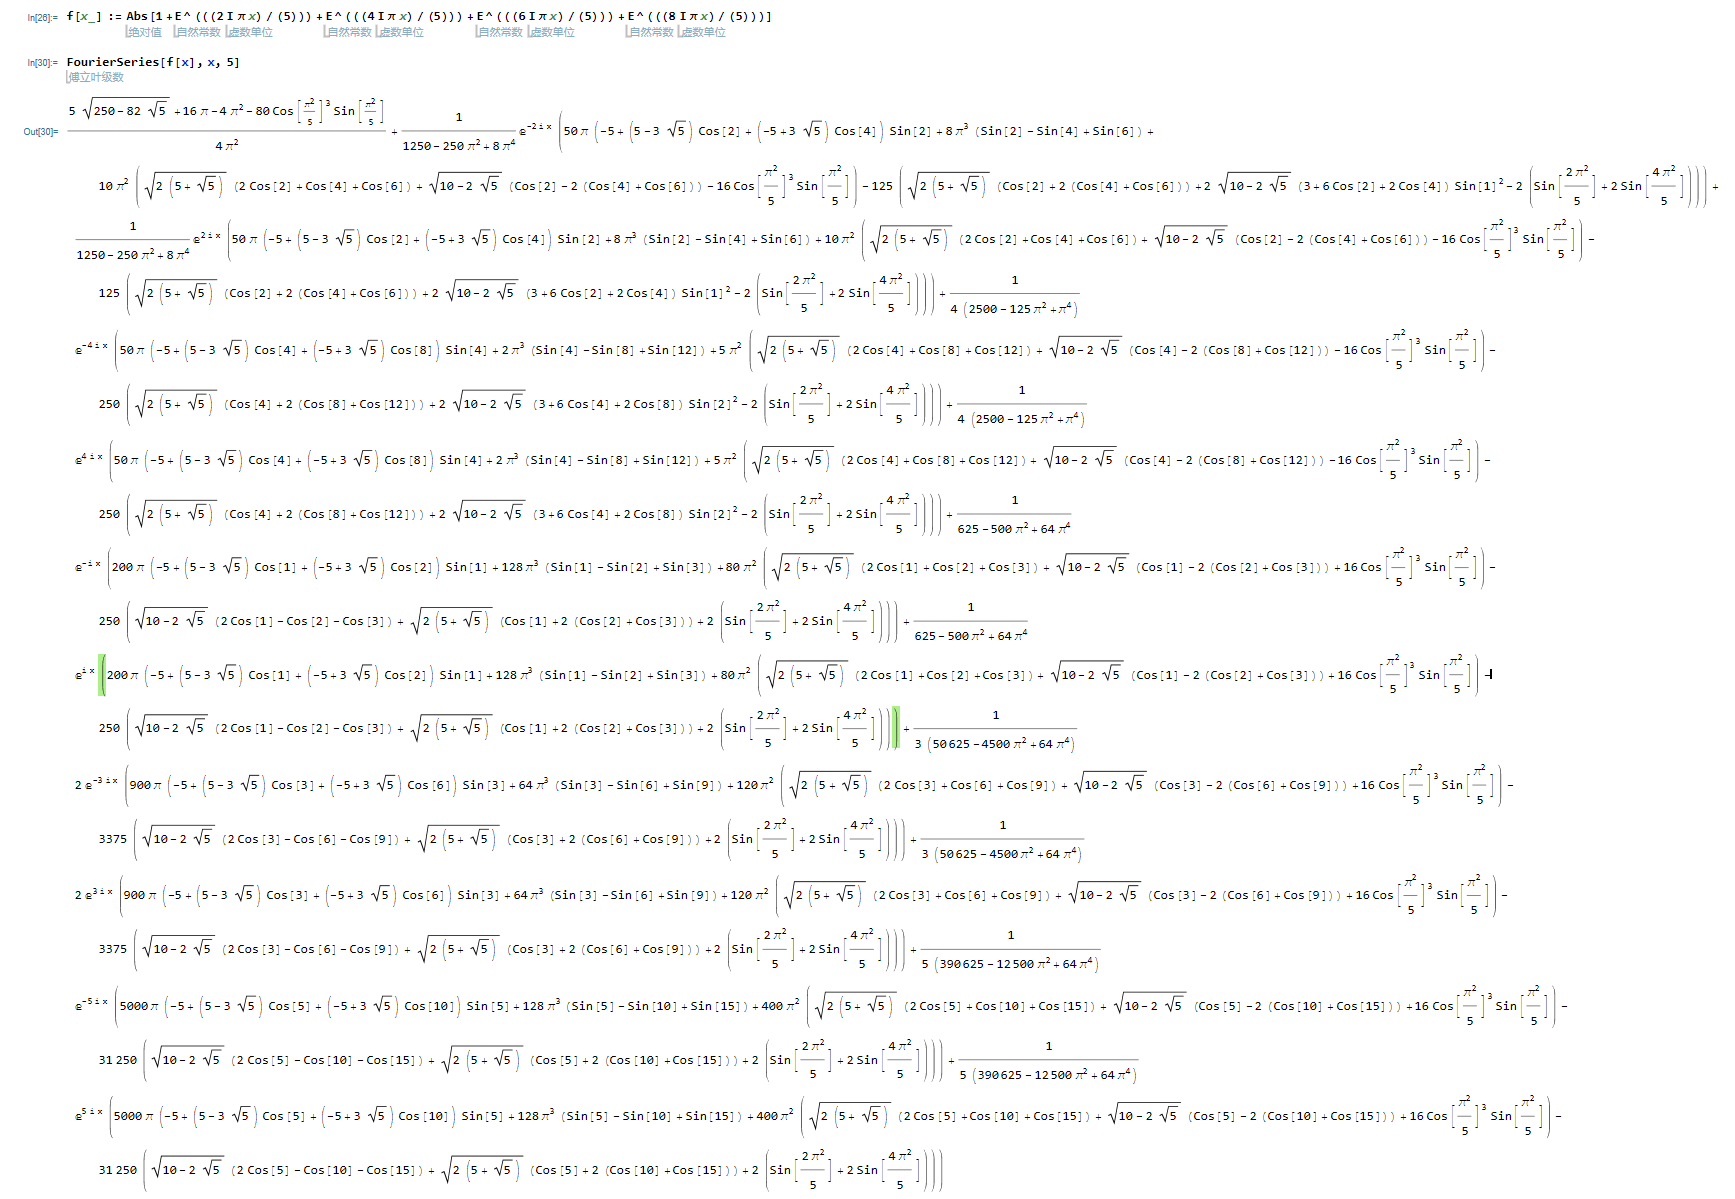
\includegraphics[width=360pt]{demo.png}
\end{figure}

\newpage

级数函数图像为:

\begin{figure}[h]
    \centering
    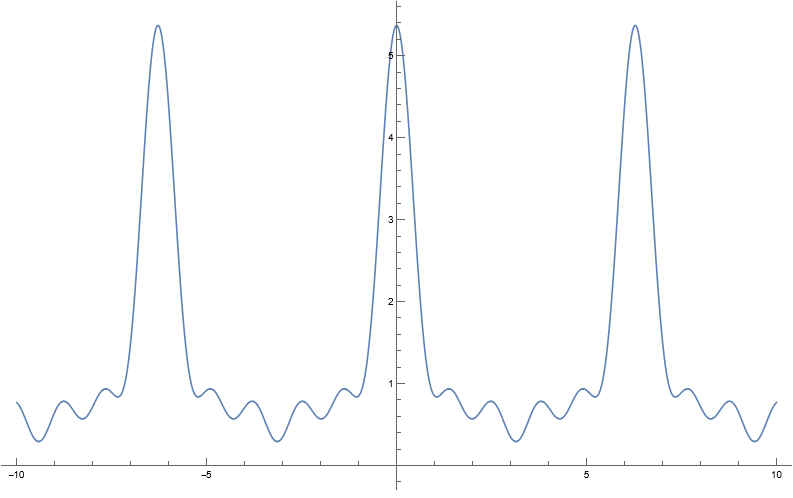
\includegraphics[width=330pt]{demo_func.png}
\end{figure}

显然,傅里叶级数展开并不能将函数简单化为几个三角函数相加的形式,计算量大(计算机运算约5分钟)且函数差距较大。

\section{结论}

一个隔项有n个零的数列(周期为k(收敛),相位为p,原数列通项公式为c)的通项公式为:

$$g(k,p,c)(n)$$

\section{推广}

对于任意周期性数列,其通项公式都可以表示成多个隔项有n个0数列的通项公式的和,也就是我们同时找到了一种任意周期性数列的通项公式。

%% The Appendices part is started with the command \appendix;
%% appendix sections are then done as normal sections
%% \appendix

%% \section{}
%% \label{}

%% If you have bibdatabase file and want bibtex to generate the
%% bibitems, please use
%%
%%  \bibliographystyle{elsarticle-num} 
%%  \bibliography{<your bibdatabase>}

%% else use the following coding to input the bibitems directly in the
%% TeX file.

\begin{thebibliography}{00}

%% \bibitem{label}
%% Text of bibliographic item

\bibitem{b1} 谭杰锋; 郑爱武. 高等数学. 清华大学出版社; 北京交通大学出版社. 2007. ISBN 978-7-8108-2647-1
\bibitem{b2} Andreescu T ,  Feng Z . 102 combinatorial problems. 2003.ISBN 978-0-8176-4317-1

\end{thebibliography}
\end{document}
\endinput
%%
%% End of file `elsarticle-template-num.tex'.
